\documentclass[12pt]{article}
\usepackage[english]{babel}
\usepackage[utf8x]{inputenc}
\usepackage{amsmath}
\usepackage{graphicx}
\usepackage[a4paper]{geometry}

\begin{document}
\begin{titlepage}

% definition of custom command for horizontal lines
\newcommand{\HRule}{\rule{\linewidth}{0.5mm}}

\center
% HEADING
\textsc{\LARGE University of Dublin,\\Trinity College}\\[1.0cm]

\includegraphics[width=0.2\textwidth]{logo.png}

\HRule \\[0.4cm]
\textsc{\Large Dice Investigation}\\[0.25cm]
\textsc{\large ST2004 \& ST2353 Assessment 1}\\[0.1cm]
\HRule \\[0.4cm]
 
% AUTHORS
\begin{minipage}{0.5\textwidth}
\begin{flushleft} \large
\emph{Authors:}
\\Alexandru \textsc{Sulea} 12315152
\\Edmond \textsc{O'Flynn} 12304742
\\Jonathan \textsc{Lester} 12345678
\\Ronan \textsc{Campbell} 12345678
\end{flushleft}
\end{minipage}
~
\begin{minipage}{0.4\textwidth}
\begin{flushleft} 
\large
\emph{Lecturer:} \\
Dr. Brett \textsc{Houlding}
\vspace{1.9cm}
\end{flushleft}
\end{minipage}\\[2cm]

% DATE
{\large \today}\\[1cm] 

% LOGO
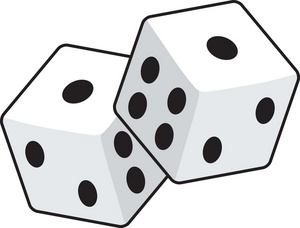
\includegraphics[width=0.3\textwidth]{dice.png}
\clearpage
\end{titlepage}

\tableofcontents
\listoffigures
\addcontentsline{toc}{section}{List of Figures}
\listoftables
\addcontentsline{toc}{section}{List of Tables}
\addcontentsline{toc}{section}{References}
\thispagestyle{empty}
\cleardoublepage
\setcounter{page}{1}

\section{Q1i: Simulation of Probability Distributions}
\subsection{Univariate System Model}
\subsection{Long Run Averages}
\subsection{Covariance}
\subsection{Condition Distribution of S3}
\clearpage

\newgeometry{top=1cm,left=1cm,bottom=2cm,right=1cm}
\section{Q1ii: Probability Distributions}
\subsection{Probability Distribution}
Three dice can be rolled in a variety of 216 ways (6*6*6) over a probability distribution shown below. The possible combinations for each die results in varied probabilities for each number, where a greater number of combinations results in a higher probabilistic outcome, and thus over the long run, results in a variance of probabilities for each dice combination. The probability of each number rolled tends from the value of the number of combinations that can be possibly formed for that combination, with respect to the total number of combinations possible for n dice.
\begin{table}[h]
\centering
\begin{tabular}{llllllll}
Sum & \multicolumn{5}{l}{Dice Combinations}  & Combinations & Probability \\
3            & 1,1,1 &        &       &       &       & 1                  & 0.005       \\
4            & 1,1,2 &        &       &       &       & 3                  & 0.014       \\
5            & 1,2,2 & 1,1,3  &       &       &       & 6                  & 0.028       \\
6            & 1,1,4 & 1,2,3  & 2,2,2 &       &       & 10                 & 0.046       \\
7            & 1,1,5 & 1,2,4  & 1,3,3 & 2,2,3 &       & 15                 & 0.069       \\
8            & 1,1,6 & 1,2,5  & 1,3,4 & 2,2,4 &       & 21                 & 0.097       \\
9            & 1,3,5 & 1,4,4  & 1,2,6 & 2,2,5 & 3,3,3 & 25                 & 0.116       \\
10           & 1,3,6 & 1,4,5  & 2,2,6 & 2,3,5 & 3,3,4 & 27                 & 0.125       \\
11           & 1,4,6 & 1,5,5  & 2,3,6 & 2,4,5 & 3,4,4 & 27                 & 0.125       \\
12           & 1,5,6 & 2,4,6, & 2,2,5 & 3,3,6 & 4,4,4 & 25                 & 0.116       \\
13           & 1,6,6 & 2,5,6  & 3,5,5 & 3,4,6 &       & 21                 & 0.097       \\
14           & 2,6,6 & 3,5,6  & 4,4,6 & 4,5,5 &       & 15                 & 0.069       \\
15           & 3,6,6 & 4,5,6  & 5,5,5 &       &       & 10                 & 0.046       \\
16           & 4,6,6 & 5,5,6  &       &       &       & 6                  & 0.028       \\
17           & 5,6,6 &        &       &       &       & 3                  & 0.014       \\
18           & 6,6,6 &        &       &       &       & 1                  & 0.005       \\
             &       &        &       &       &       & 216                & 1          
\end{tabular}
\caption{Probability Distribution of Combinations}
\end{table}
\subsection{Multinomial Theorem}
The multinomial theorem is a \emph{generating function} by which a probability distribution of dice sums may be calculated and expressed. The series is defined by the power of the number, where the exponent itself is a polynomial with respect to the number rolled by the die for any positive integer m and non-negative integer n.
$$(x_1+x_2+...+x_m)^n=\sum_{k_1+k_2+...+k_m=n}{}\frac{n!}{k_1!k_2!...k_m!}\prod_{1\leq t\leq m}^{}x_{t}^{k_t}$$
In the case of $S_n$ where n dice of 6 sides have been rolled
$$G(S_n)=\left(\sum_{k=1}^{6}x^k\right)^n=(x^1+x^2+x^3+x^4+x^5+x^6)^n$$
Such that for multiple dice
\begin{align*}
G(S_1)&=x^1+x^2+x^3+x^4+x^5+x^6\\
G(S_2)&=(x^1+x^2+x^3+x^4+x^5+x^6)^2\\
&=x^2+2x^3+3x^4+4x^5+5x^6+6x^7+5x^8+4x^9+3x^{10}+2x^{11}+x^{12}
\end{align*}

\subsection{Expected Value and Variance}
Expected value is defined as the product of given value with respect to thte probabilistic outcome of that value, as a summation of all the possible values  within that set for a randomly distributed variable X:
\begin{align*}
E[X_n]=x_np_n \quad \textrm{where} \quad E[X]=\sum_{i=1}^{n}x_np_n
\end{align*}
Given the probability distribution, the expected value is calculated as such:
$$E[X]=1*\frac{1}{6}+1*\frac{2}{6}+1*\frac{3}{6}+1*\frac{4}{6}+1*\frac{5}{6}+1*\frac{6}{6}=3.5$$
In the case of having three dice, this method can be extended to encapsulate a wider range of values over two additional dice:
$$E[X]=3*\frac{1}{216}+4*\frac{3}{216}+5*\frac{6}{216}+6*\frac{10}{216}+7*\frac{15}{216}+8*\frac{21}{216}+9*\frac{25}{216}+10*\frac{27}{216}+$$
$$11*\frac{27}{216}+12*\frac{25}{216}+13*\frac{21}{216}+14*\frac{15}{216}+15*\frac{10}{216}+16*\frac{6}{216}+17*\frac{3}{216}+18*\frac{1}{216}$$\\
The rolling of dice in such a way is denoted as an independent event, as the dice rolls in the future are not dependent on previous rolls and do not affect the outcome of values, where essentially the expected outcome of the event is given by:
$$E[X+Y+Z]=E[X]+E[Y]+E[Z]$$
Given the independence of each die roll, the expected value for three rolls is given by:
$$E[X+Y+Z]=3.5+3.5+3.5=10.5$$
Thus confirming the supposition by applying probabilistic arguments to the real-world. Ergo, variance of a random variable is denoted by the following:
\begin{align*}
\sigma^2(X)&=E[(X-\mu)^2]\\
&=E[X^2-2XE[X]+E(X)^2]\\
&=E[X^2]-2E[X]E[X]+(E[X])^2\\
&=E[X^2]-(E[X])^2
\end{align*}
Therefore the variance for the set can be determined from the above equations results in the following using the square of the value rolled from 1-6 a total of 1 time:
$$E[X^2]=1*\frac{1}{6}+4*\frac{1}{6}+9*\frac{1}{6}+16*\frac{1}{6}+25*\frac{1}{6}+36*\frac{1}{6}=15.16$$
$$\sigma^2(X)=15.16-(3.5)^2=2.91$$
Given the joint probabilities via S3, S4, M3 and N4; the expected value of M3 is the sum-product of the marginal probability of M3. The same is true for the expected value of M4 with respect to M4 itself. Thus,
$$E[M3]=0.005+0.065+0.264+0.630+1.481+2.529=4.972$$
Similar to one die, calculating the sum of three dice results in a similar manner:
\begin{align*}
E[X^2]&=9*\frac{1}{216}+16*\frac{3}{216}+49*\frac{6}{216}+64*\frac{10}{216}+81*\frac{15}{216}+100*\frac{21}{216}\\&+121*\frac{27}{216}+144*\frac{27}{216}+169*\frac{21}{216}+196*\frac{15}{216}+225*\frac{10}{216}\\&+256*\frac{6}{216}+289*\frac{3}{216}+324*\frac{1}{216} = 119\\
\sigma^2(X)&=119-(10.5^2)=8.75
\end{align*}
For each given roll, there is independence between variables. Therefore the total variance is the sum of the individual variances within the set:
\begin{align*}
\sigma^2(S3)&=\sigma^2(X1)+\sigma^2(X2)+\sigma^2(X3)\\
&=2.91+2.91+2.91=8.73\approx8.75
\end{align*}
\begin{align*}
\centering
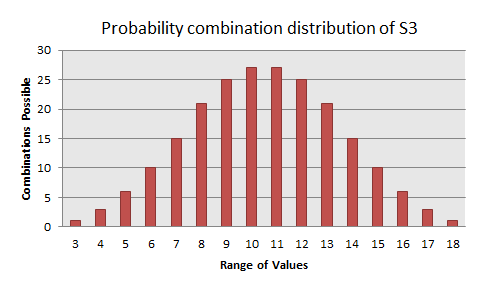
\includegraphics[width=0.5\textwidth]{PD_S3.png}
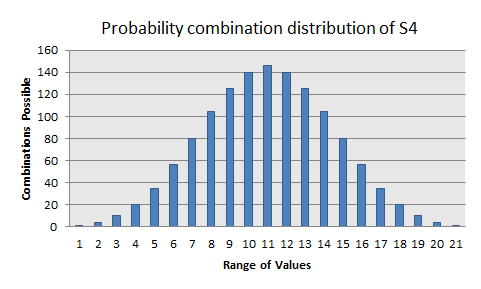
\includegraphics[width=0.5\textwidth]{PD_S4.png}
\end{align*}
\subsection{Covariance}
Covariance in a dataset is a measure of how much two random variables change together within a given time. Covariance within the data sets may be defined as followed
\begin{align*}
\sigma(X,Y)&=E[(X-E(X))(Y-E(Y))]\\
&=E[XY-XE(Y)-Y(EX)+E(X)E(Y)]\\
&=E(XY)-E(X)E(Y)-E(Y)E(X)+E(X)E(Y)\\
&=E(XY)-E(X)E(Y)
\end{align*}
Thus calculating $\sigma(S3,M3)$ for the joint probabilities of (S3,M3) and (S4,M4) respectively gives
\begin{align*}
\sigma(S3,M3)&=54.764-(4.972*(3*3.5))=2.558\\
\sigma(S4,M4)&=74.589-(5.181*(4*3.5))=2.055
\end{align*}

\subsection{Long Run Expected Values and Variances}
Following the \emph{Central Limit Theorem} which implies that $X_1,X_2,...,X_n$ are all independent random variables, where each random variable within the set pertains to tending to the same expected value, $\mu$, and standard deviation, $\sigma^2$, within the distribution given that the population is sufficiently large with n values of dice summation.
\begin{align*}
\centering
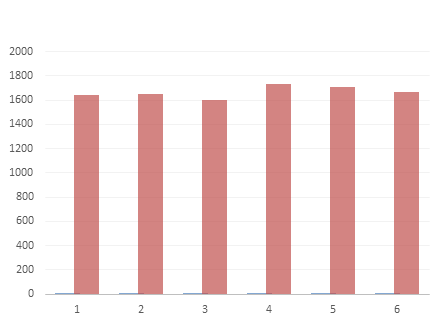
\includegraphics[width=0.5\textwidth]{s1.png}
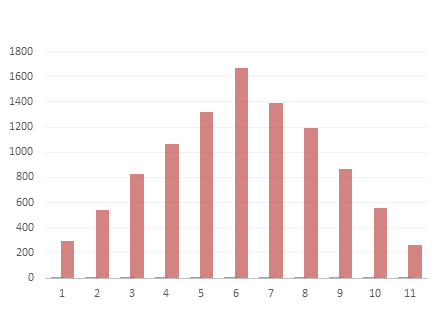
\includegraphics[width=0.5\textwidth]{s2.png}
\end{align*}
\begin{align*}
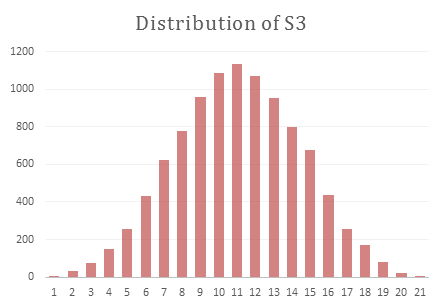
\includegraphics[width=0.5\textwidth]{s3.png}
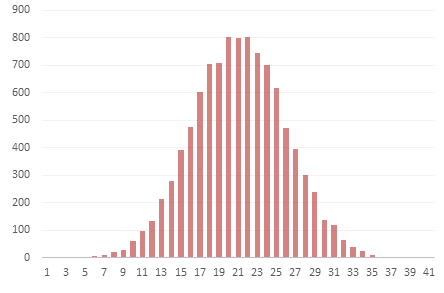
\includegraphics[width=0.5\textwidth]{s4.png}
\end{align*}
The above charts are $S_1$, $S_2$, $S_4$, and $S_8$ which demonstrate the effects of tending to the normal distribution curve as n samples approaches infinity.  Ergo, the expected value of $E[S_k]$ is therefore shown to be $E[S_k]=K*E[S_1]$, while the expected long run variance $V[S_k]$ is shown to be $V[S_k]=K*V[S_k]$
\clearpage

\section{Q1iii: Law of Large Numbers}
\subsection{Comparison}
\clearpage

\section{Q2: Investigation}
\subsection{Q2}
\clearpage

\end{document}
